\section{Software evolution}
\begin{table}[H]
\caption{Evolution spiral}
\begin{center}
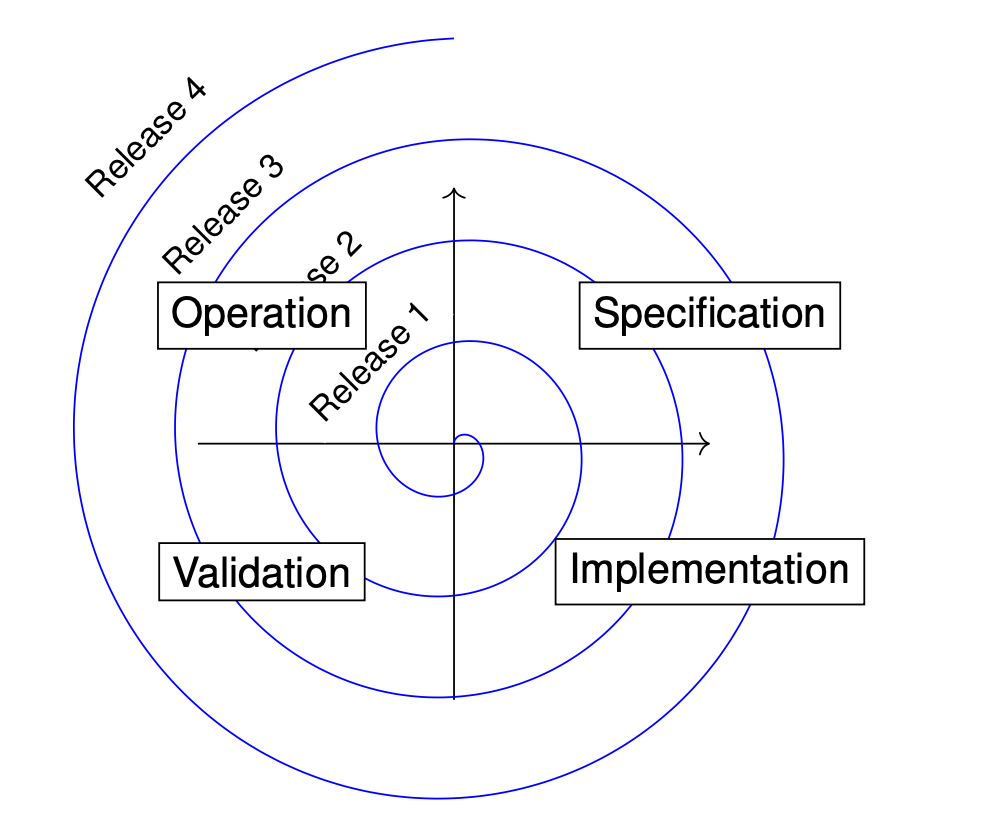
\includegraphics[scale=0.125]{Evolution_spiral.png}	
\end{center}
\end{table}
Bei Custom-Software zahlt der Kunde nur die Entwicklung und muss sich anschließend selbst um die Evolution kümmern
\begin{table}[H]
\caption{Alternative software evolution}	
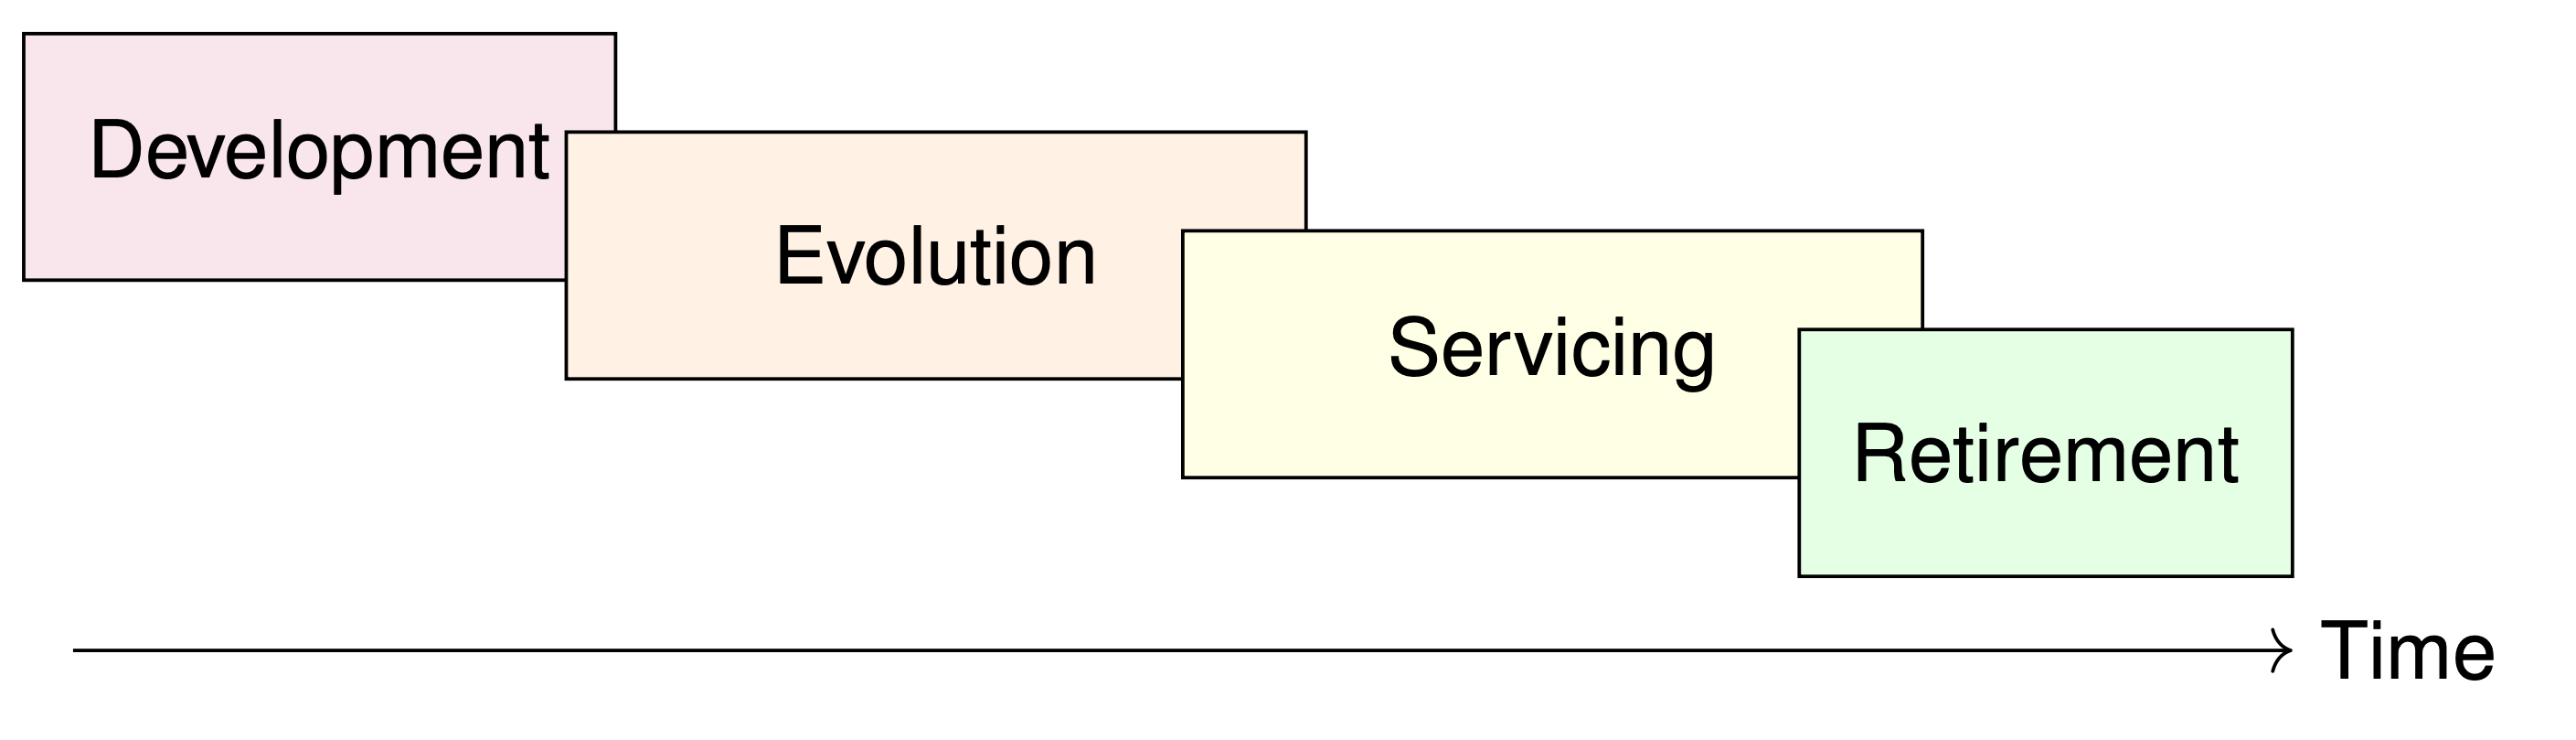
\includegraphics[scale=0.125]{Alternative_evolution.png}
\end{table}
\subsection{Evolution processes}
\begin{table}[H]
\caption{Evolution processes}
\begin{center}
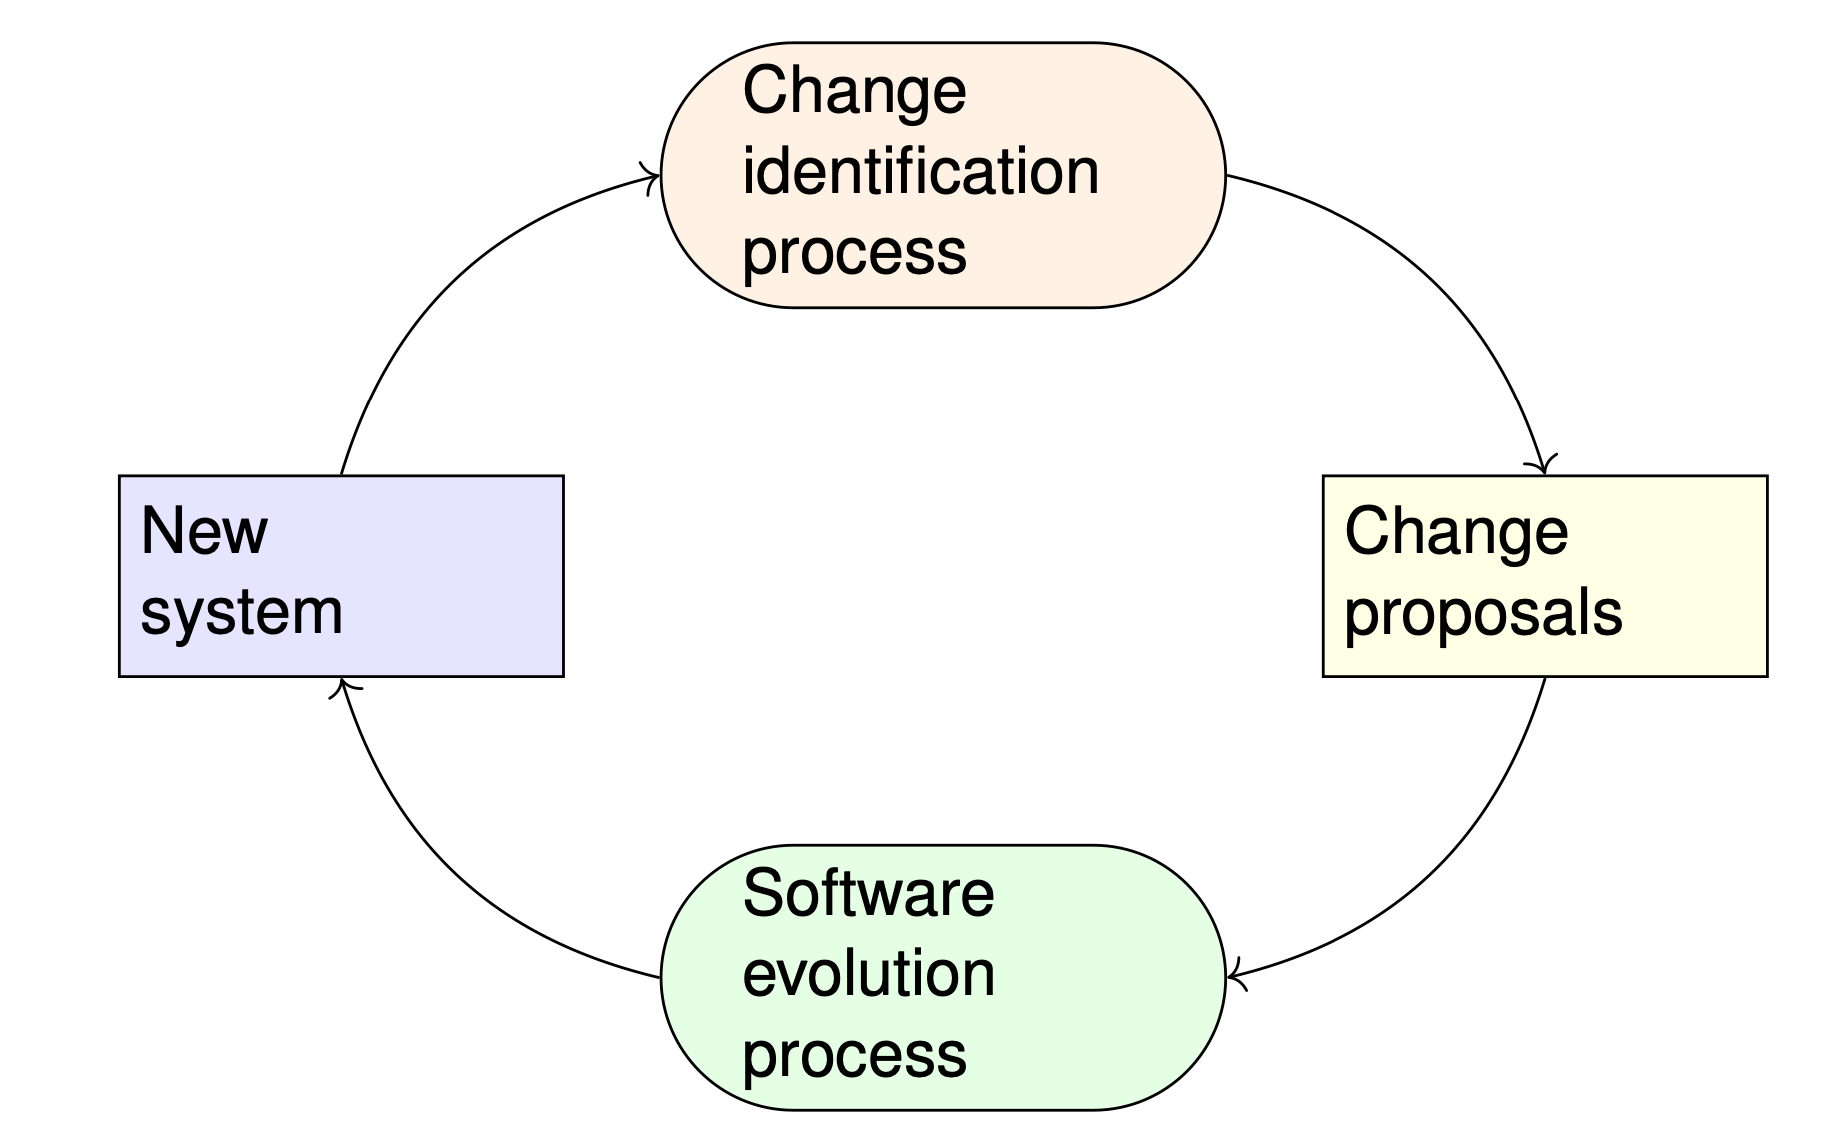
\includegraphics[scale=0.125]{Evolution_processes.png}		
\end{center}
\end{table}
\subsubsection{Generic evolution process}
\begin{table}[H]
\caption{Generic evolution model}
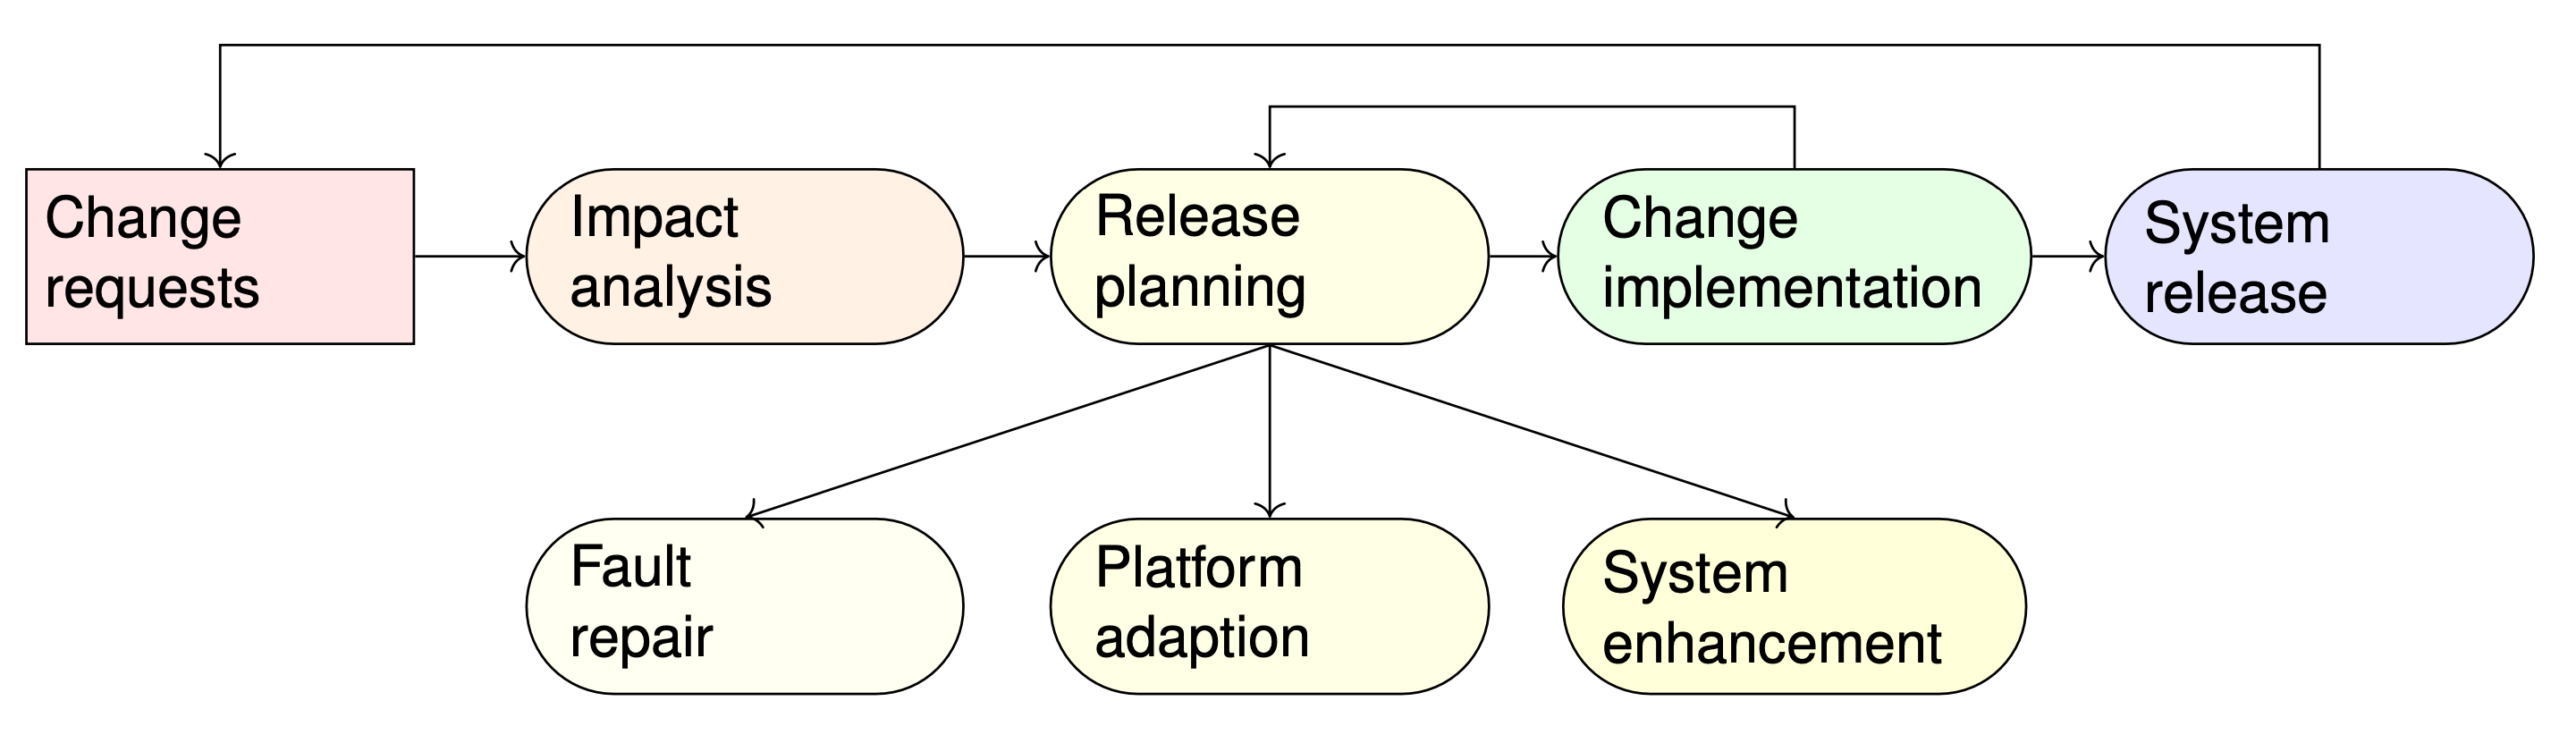
\includegraphics[scale=0.125]{Generic_evolution_model.png}	
\end{table}
\subsubsection{Emergency repair}
Nach einem Emergency repair sollte der Code refactored werden, um keine weiteren Schäden am System zu verursachen
\subsubsection{Agile vs. Plan-driven}
\begin{itemize}
	\item Agile dev \& plan-driven evolution
		\begin{itemize}
			\item Es gibt keine detaillierte Dokumentation für das Evolutionsteam
			\item Klar definierte Anforderungen existieren möglicher Weise nicht
		\end{itemize}
	\item Plan-driven dev \& agile evolution 
		\begin{itemize}
			\item Evolutionsteam muss automatisierte Tests from scratch entwickeln
	 		\item Code ist möglicherweise nicht refactored oder simplifiziert
 		\end{itemize}
\end{itemize}
\subsubsection{Agile}
\begin{multicols}{2}
$\bold{Pros}$:
\begin{itemize}
	\item Test-driven development
	\item Automated regression testing
	\item System changes as user stories
\end{itemize}
\columnbreak
$\bold{Cons}$:
\begin{itemize}
	\item Nutzer ins Entwicklungsteam involvieren ist praktisch unmöglich
	\item Emergency repairs könnten Entwicklungszyklen unterbrechen
	\item Abstand zwischen Releases könnte vergrößert werden, um den Operationsprozess nicht zu stören 
\end{itemize}
\end{multicols}
\subsection{Software maintenance}
\subsection{Types of maintenance}
\begin{itemize}
	\item Fault repair
	\item Environmental adaption
	\item Functionality addition
\end{itemize}
In der maintenance Phase ist das entwickeln von neuen Funktionen teurer, weil sich ein neues Team in den Code einarbeiten müsste
\subsubsection{Maintenance prediction}
Versucht vorherzusagen, welche Veränderungen nötig sind und wie teuer dies werden
\subsubsection{Software reengineering}
Reengineering ermöglicht eine bessere Struktur, Verständnis und Maintainability, bei legacy Systemen\newline
Es könnte
\begin{itemize}
	\item Redocumentation
	\item Refactoring
	\item Translating in modern languages
	\item Modifying structures and values 
\end{itemize}
umfassen und reduziert Risiken und Kosten
\begin{table}[H]
\caption{Reengineering}	
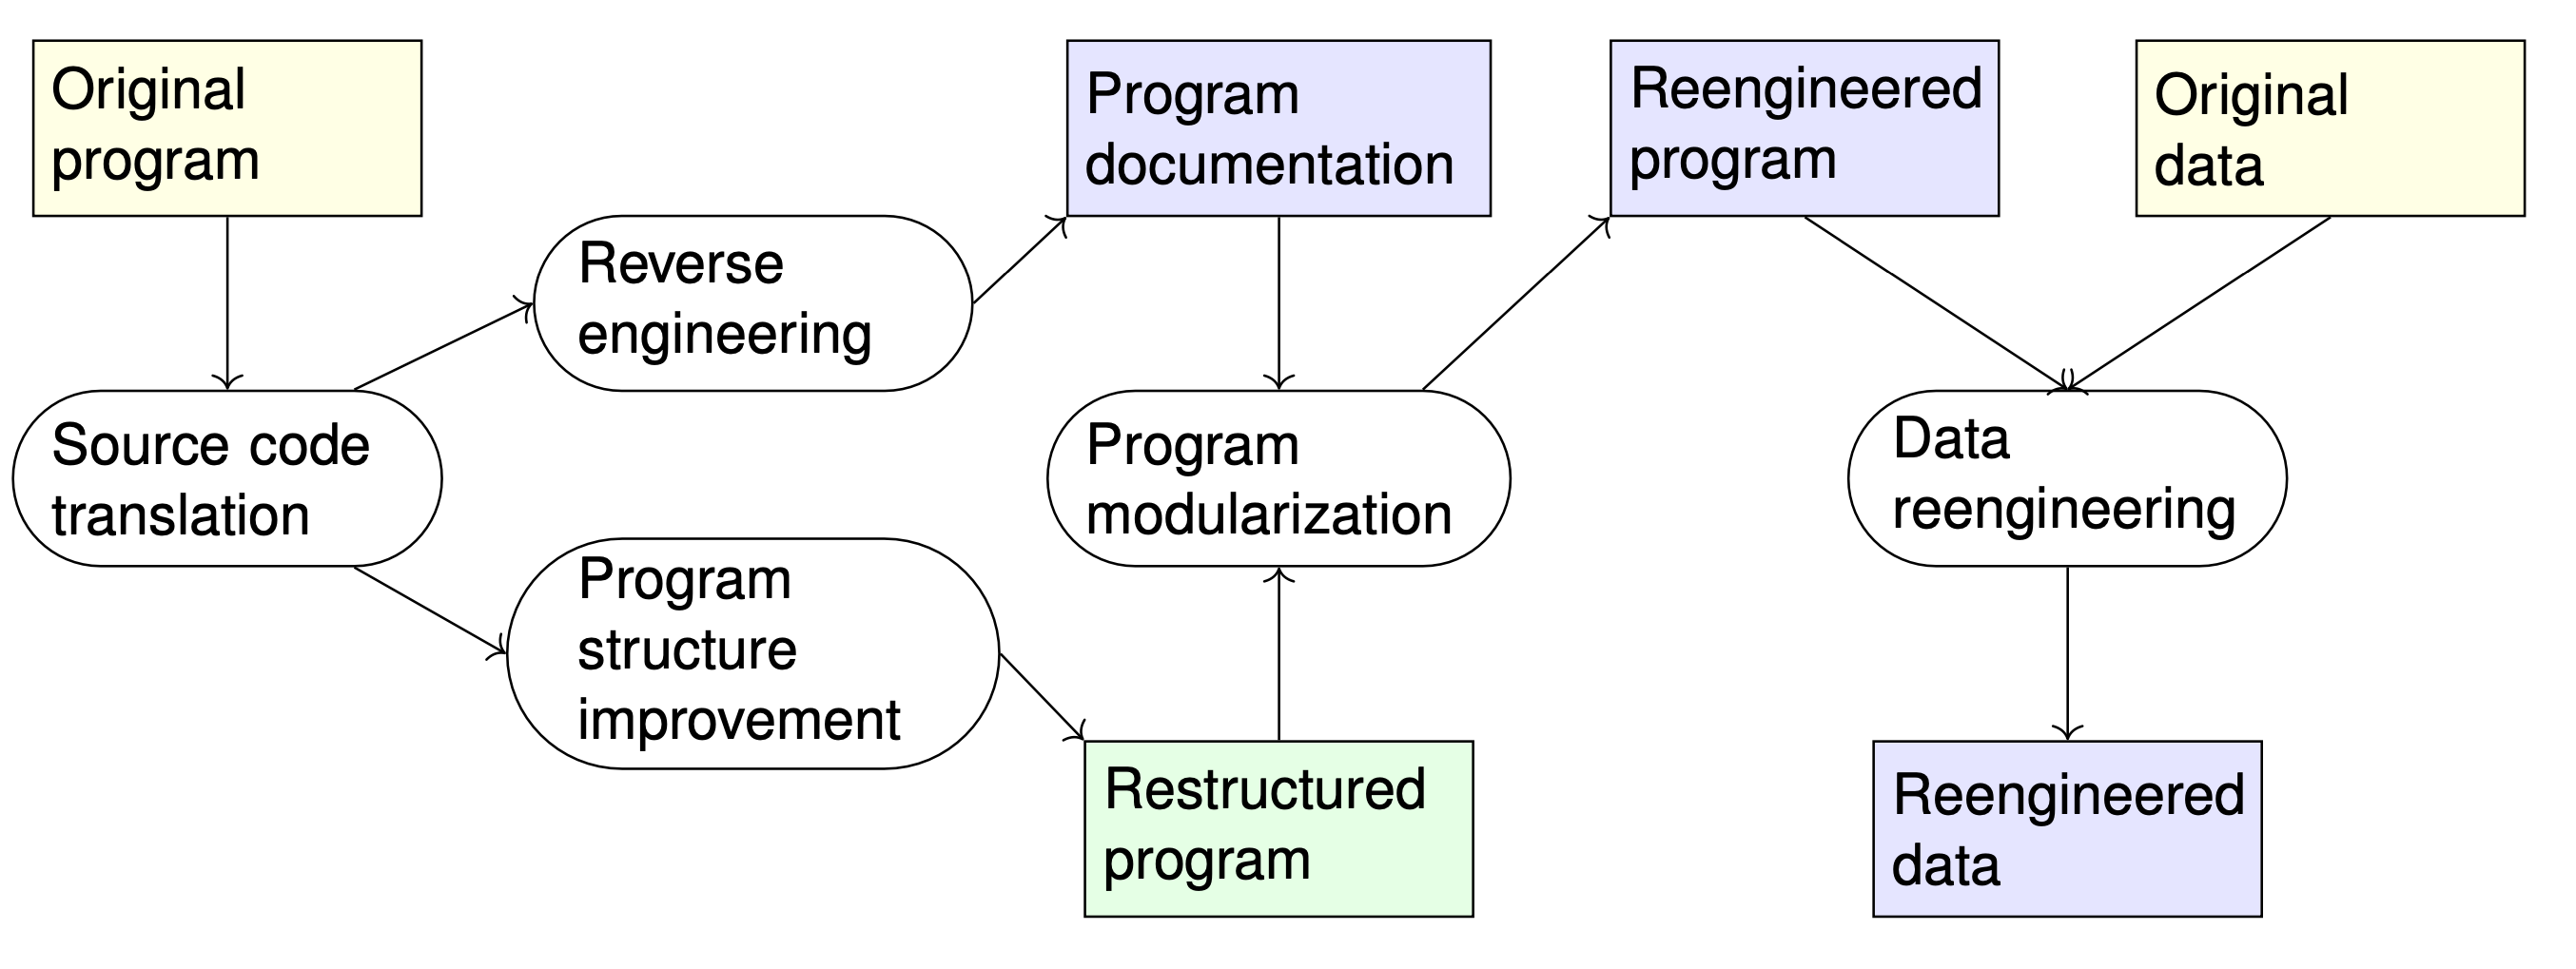
\includegraphics[scale=0.125]{Reengineeering.png}
\end{table}
$\bold{Cons}$:
\begin{itemize}
	\item Funktional kann nicht in objektorientiert umgewandelt werden
	\item Scher zu automatisieren
	\item Nicht so maintainable wie neue Systeme
\end{itemize}
\subsubsection{Refactoring}
\begin{itemize}
	\item Code duplicates $\to$ One function
	\item Long methods $\to$ More shorter functions
	\item Switch case statements $\to$ Polymorphism
	\item Data clumping $\to$ One object, that encapsulates all data
	\item Speculative generality $\to$ Remove not used generality
\end{itemize}
\subsection{Legacy systems}
Alte Systeme, die auf veralteten Sprachen und veralteter Technologie basieren
\subsubsection{Problems}
\begin{itemize}
	\item System hardware
	\item Support software
	\item Application software
	\item Application data
	\item Business process
	\item Business policies and rules
\end{itemize}
\begin{table}[H]
\caption{Legacy systems}
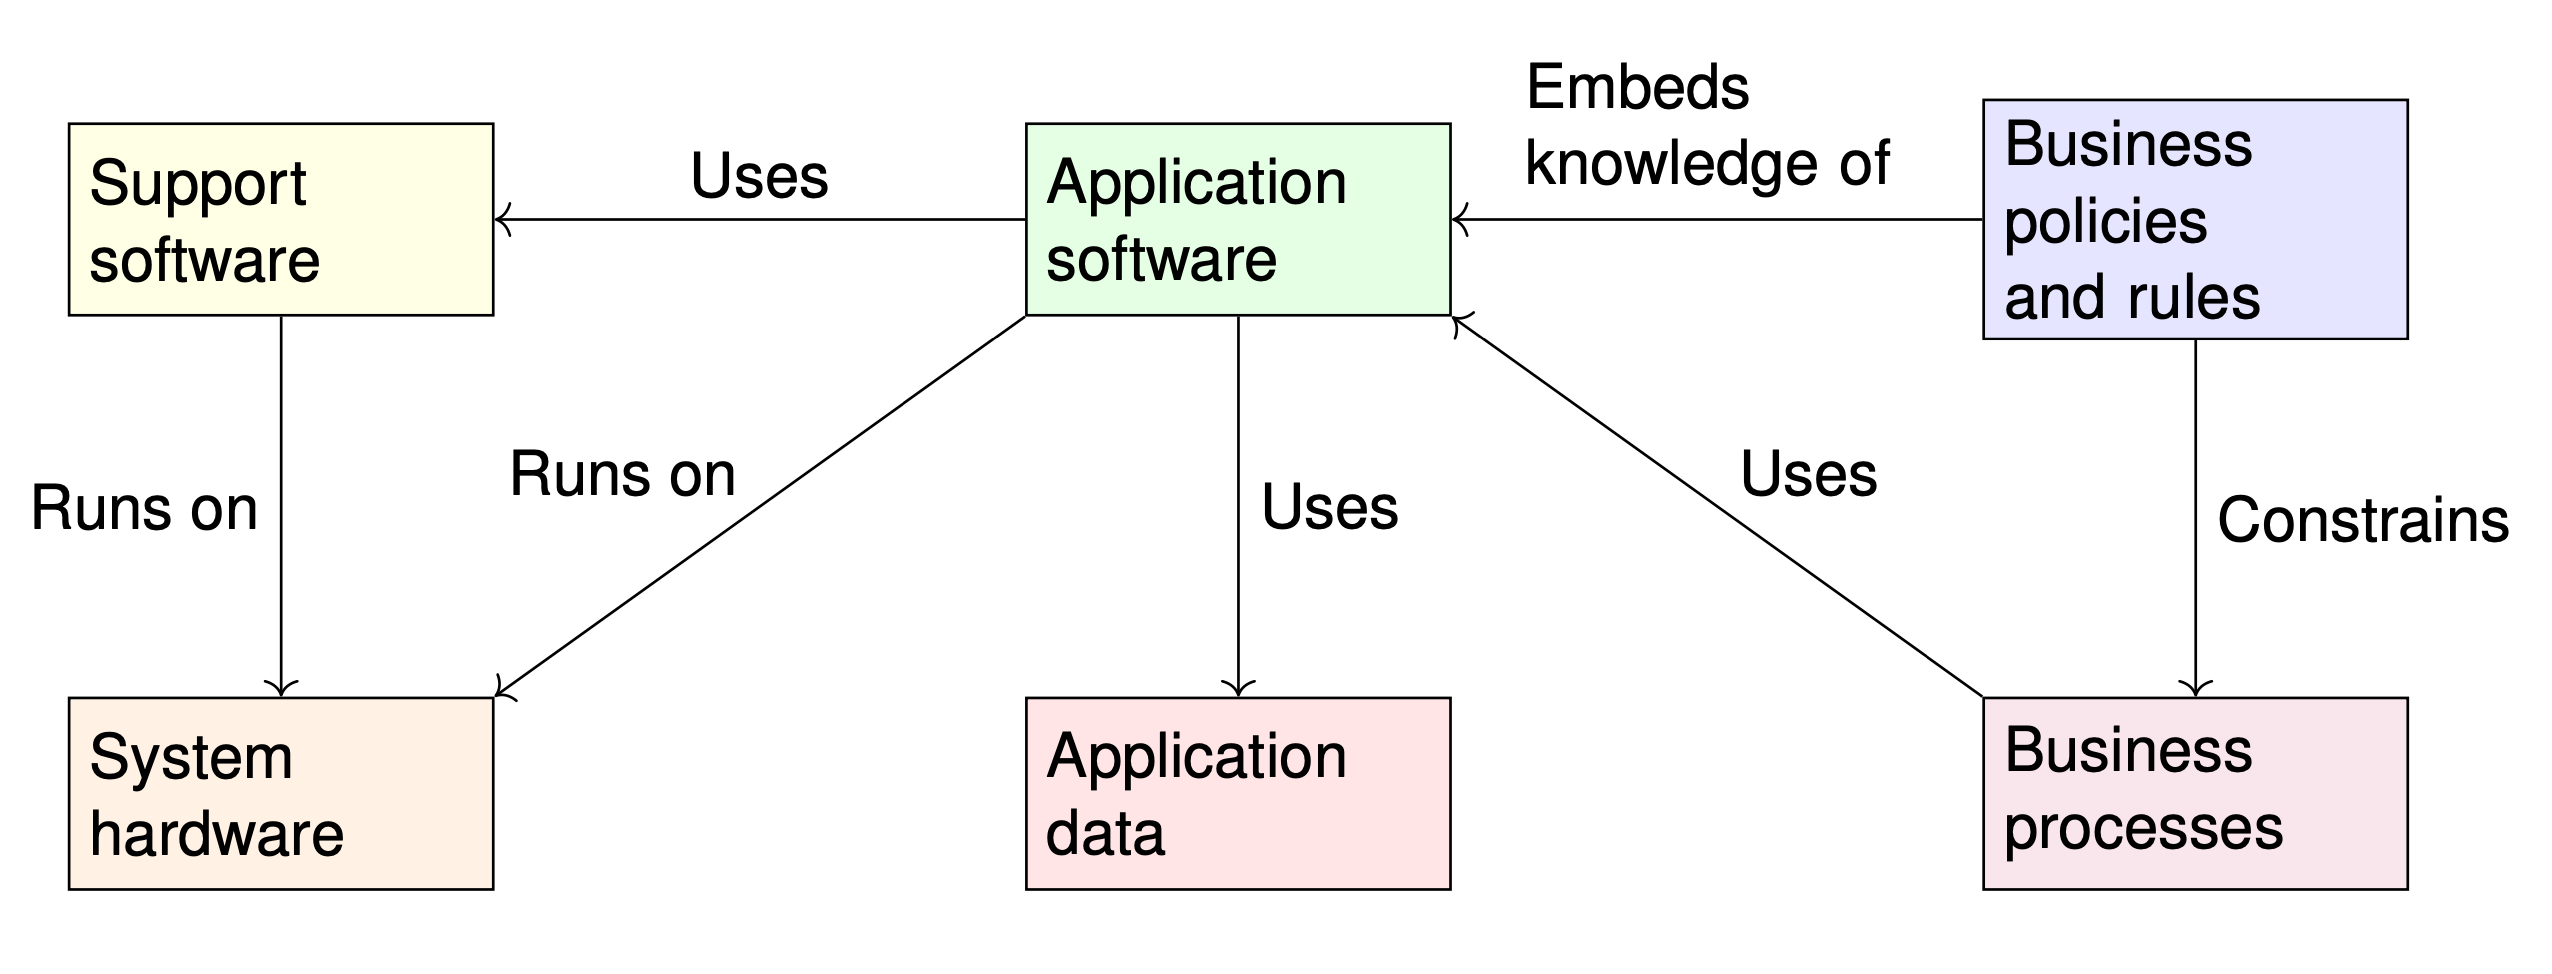
\includegraphics[scale=0.125]{Lecay.png}	
\end{table}
\subsubsection{Why so expensive}
\begin{itemize}
	\item Inkonsistente Programmierstyles und Konventionen $\to$ schwer zu verstehen
	\item Veraltete Sprachen $\to$ Erfordern Spezialisten
	\item Veraltete oder nicht vorhandene Dokumentation
	\item Struktur hat wegen Maintenance gelitten
	\item Optimierungen für alte Hardware erschweren Verständlichkeit 
	\item Daten können Mengel aufweisen
\end{itemize}
\subsubsection{Strategies}
\begin{itemize}
	\item Vollständig entfernen
	\item Weiter maintainen
	\item Reengineering
	\item Ersetze Teile oder komplett
\end{itemize}





